\documentclass[aspectratio=169]{beamer}

\usepackage[T1]{fontenc}
\usepackage[magyar]{babel}
\usepackage{hyperref}
\usepackage{biblatex}
\usepackage{csquotes}
\usepackage{graphicx}

\setbeamertemplate{navigation symbols}{}
%\setbeamertemplate{footline}[frame number]
\setbeamertemplate{caption}{\insertcaption}

\usetheme{Madrid}
\usecolortheme{default}
\renewcommand{\figurename}{}
\newcommand{\framet}{\frametitle{\secname{} - \subsecname}}

\begin{document}
\title{Atomerő-mikroszkóp és pásztázó alagútmikroszkóp}
\subtitle{AFM és STM}
\author{Készítette: Illés Gergő}
\date{2023. április 24.}
\begin{frame}
\maketitle
\end{frame}
\begin{frame}
\frametitle{Tartalomjegyzék}

\begin{columns}
\column{.90\textwidth}
\tableofcontents
\end{columns}
\end{frame}

\section{Atomerő mikroszkópia}
\subsection{Történeti áttekintés}
\begin{frame}
\frametitle{\secname{} - \subsecname}
\begin{minipage}[m]{0.63\linewidth}
\begin{itemize}
\item Pásztázószondás-mikroszkópia
\item Abbe-féle diffrakciós limit $d=0,61\dfrac{\lambda}{N_A}$
\item Gerd Binnig, Calvin Quate és Christopher Gerber
\item Demonstráció: 1986
\end{itemize}
\end{minipage}
\hfill
\begin{minipage}[m]{0.36\linewidth}
\begin{figure}
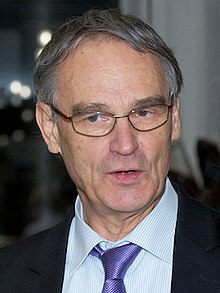
\includegraphics[width=0.7\textwidth]{gerd.jpg}
\caption{Gerd Binnig}
\end{figure}
\end{minipage}
\end{frame}
\subsection{Elméleti áttekintés}
\begin{frame}
\frametitle{\secname{} - \subsecname}
\begin{minipage}{.60\linewidth}
\begin{itemize}
\item Laprugó tűvel a végén
\item Erőhatások: Coulomb-erő, van der Waals erők
\item Piezzo-elektromos mozgatók
\item Fotodetektor
\end{itemize}
\end{minipage}
\hfill
\begin{minipage}[m]{.39\linewidth}
\begin{figure}
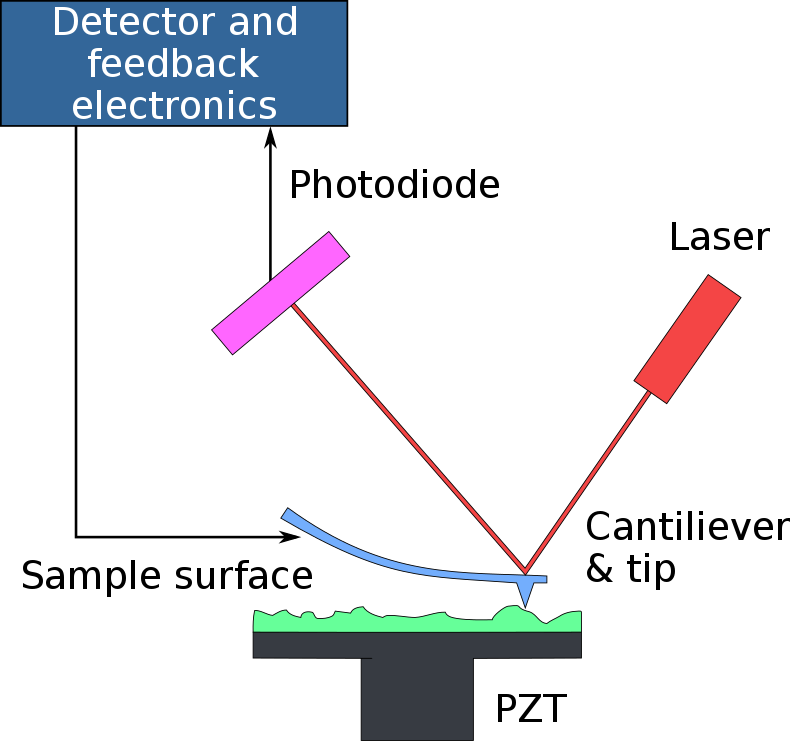
\includegraphics[width=.8\textwidth]{afm.png}
\caption{AFM sematikus rajza}
\end{figure}
\end{minipage}
\end{frame}


\begin{frame}
\begin{minipage}[m]{.49\linewidth}
\begin{figure}
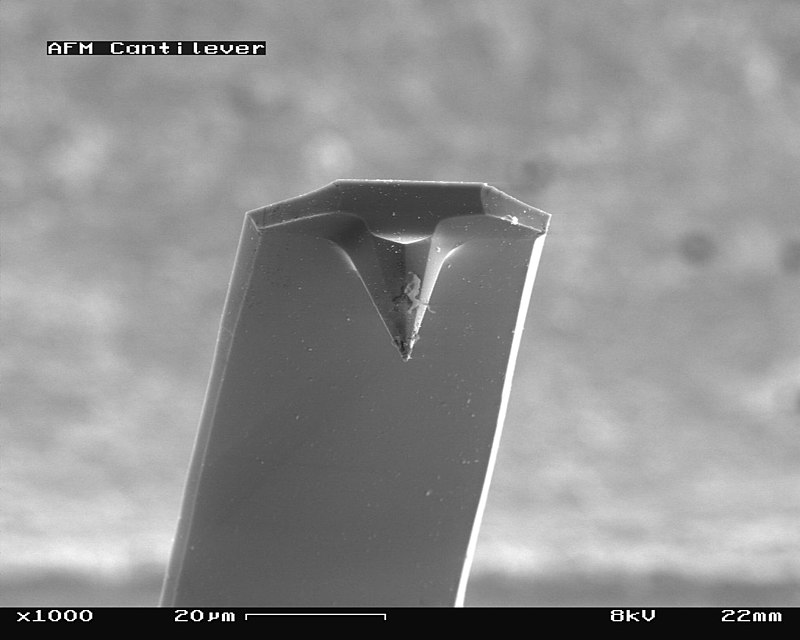
\includegraphics[width=\textwidth]{laprugo.jpg}
\caption{AFM tű elektronmikroszkóp alatt}
\end{figure}
\end{minipage}
\begin{minipage}[m]{.49\linewidth}
\begin{figure}
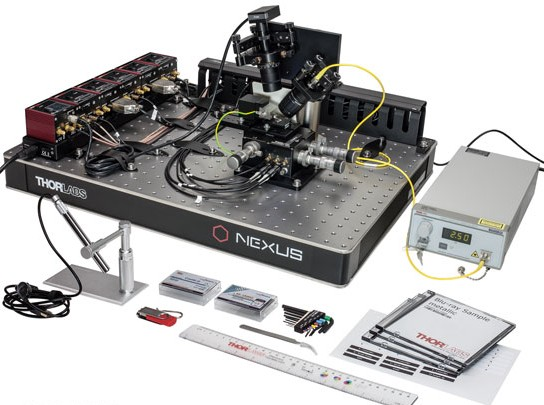
\includegraphics[width=\textwidth]{afm_thor.jpg}
\caption{Thorlabs AFM csomag}
\end{figure}
\end{minipage}
\end{frame}
\subsection{Működési üzemmódok}
\begin{frame}
\framet
\begin{itemize}
\item Kontakt mód: hajlékony laprugó, kopás
\begin{itemize}
\item Állandó magasság
\item Állandó meghajlás
\end{itemize}
\item Tapogató mód: rezonanciafrekvencia, kitérés, kisebb mértékű kopás
\item Kontakt nélküli mód: távoli erők mérése (van der Waals), legkevesebb degradáció
\end{itemize}
\end{frame}
\subsection{Felvételek}
\begin{frame}
\framet
\begin{minipage}[m]{.49\linewidth}
\begin{figure}
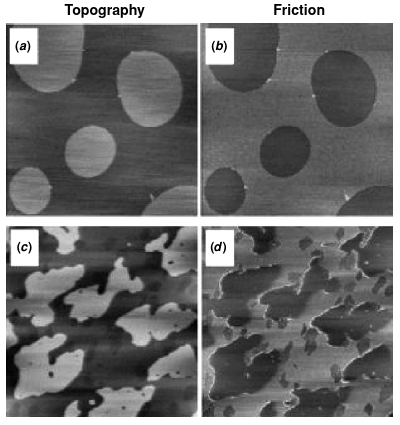
\includegraphics[width=.8\textwidth]{afm_kep1.png}
\end{figure}
\end{minipage}
\begin{minipage}[m]{.49\linewidth}
\begin{figure}
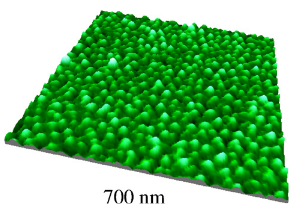
\includegraphics[width=\textwidth]{afm_kep2.png}
\end{figure}
\end{minipage}
\end{frame}

\section{Pásztázó alagútmikroszkóp}
\subsection{Történeti áttekintés}
\begin{frame}
\framet
\begin{minipage}[m]{.63\textwidth}
\begin{itemize}
\item Pásztázószondás mikroszkópia
\item Gerd Binnig, Heinrich Rohrer
\item Szabadalom: 1979
\item Nobel-díj: 1986
\end{itemize}
\end{minipage}
\hfill
\begin{minipage}[m]{.36\linewidth}
\begin{figure}
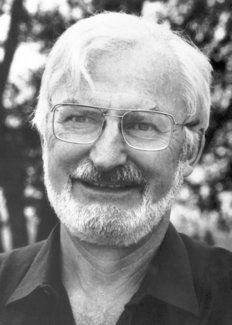
\includegraphics[width=.7\textwidth]{rohrer.jpg}
\caption{Heinrich Rohrer}
\end{figure}
\end{minipage}
\end{frame}


\subsection{Elméleti áttekintés}
\begin{frame}
\framet
\begin{minipage}[m]{.55\linewidth}
\begin{itemize}
\item Amíg az AFM elsősorban mechanikai kölcsönhatást mér az STM az elektron alagutazáson alapszik
\item Áramot mérünk a feszültség és a szonda magasságának függvényében
\item 100 pm-es felbontás oldalirányban, 10 pm-es mélységi felbontás 
\end{itemize}
\end{minipage}
\hfill
\begin{minipage}{.44\linewidth}
\begin{figure}
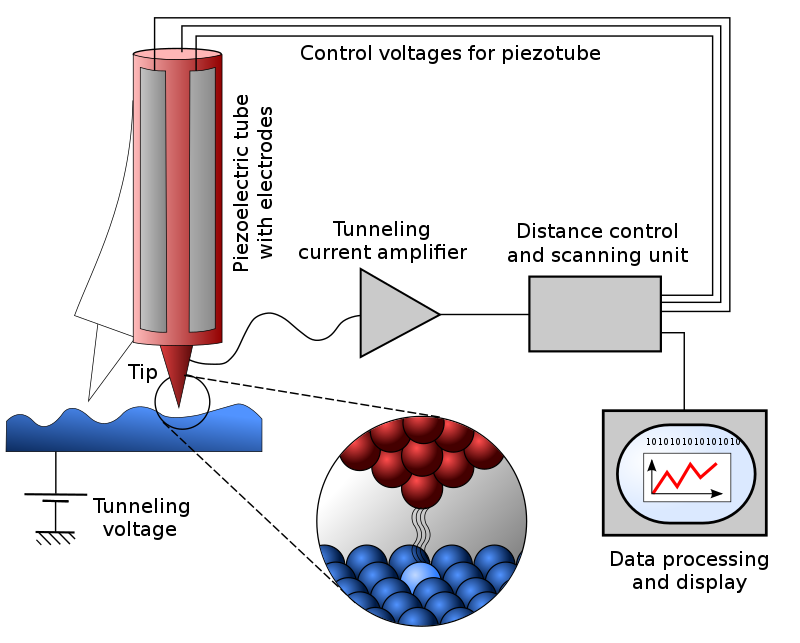
\includegraphics[width=\linewidth]{stm.png}
\caption{STM berendezés vázlata}
\end{figure}
\end{minipage}
\end{frame}
\begin{frame}
\begin{minipage}[m]{.63\linewidth}
\begin{figure}
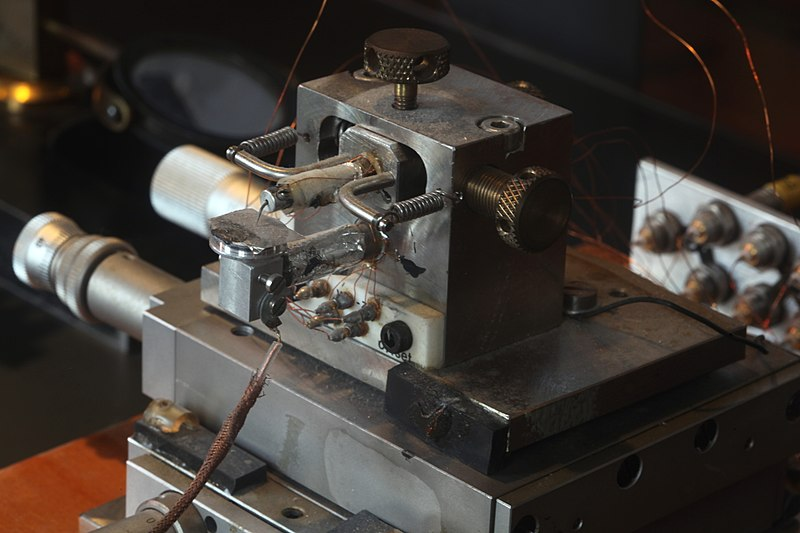
\includegraphics[width=.95\textwidth]{stm_1.jpg}
\caption{Egyik első működő STM berendezés}
\end{figure}
\end{minipage}
\begin{minipage}[m]{.36\linewidth}
\begin{figure}
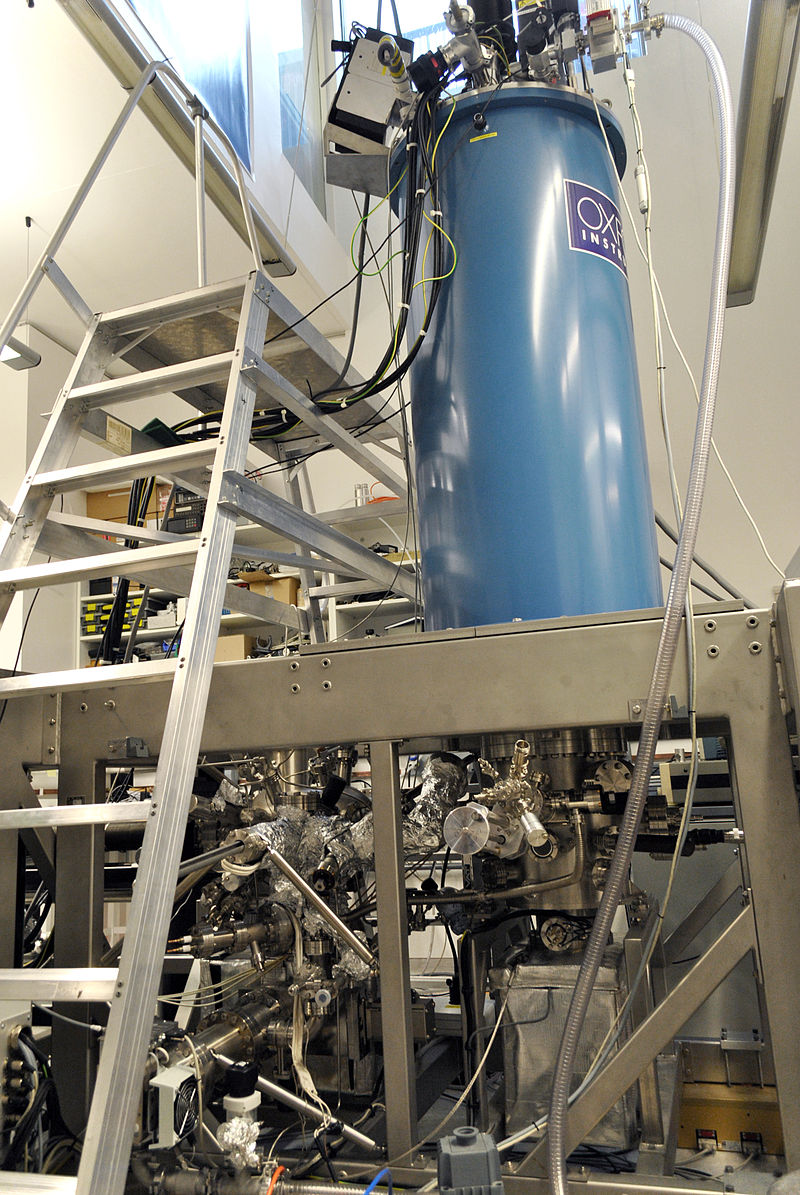
\includegraphics[width=.8\textwidth]{stm_2.jpg}
\caption{Modern STM műszer}
\end{figure}
\end{minipage}
\end{frame}
\subsection{Felhasználási lehetőségek}
\begin{frame}
\framet

\begin{columns}
\column{0.5\linewidth}
\begin{itemize}
\item Finom felületi struktúrák vizsgálata
\item Kirstály és molekulaszerkezetek
\item Defektusok keresése
\end{itemize}
\column{0.49\textwidth}
\begin{figure}
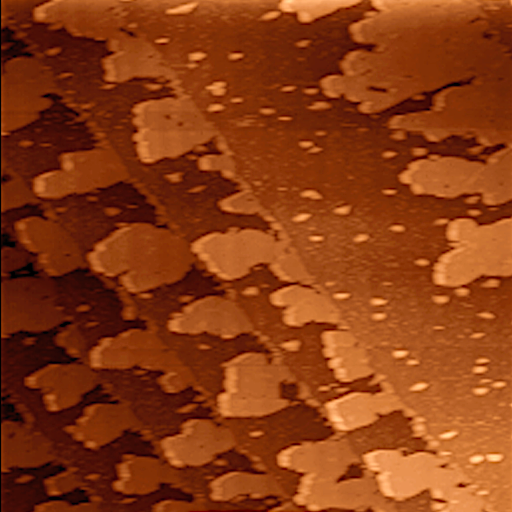
\includegraphics[width=.75\textwidth]{stm_silver.png}
\caption{Palládium kristályon növesztett ezüst szigetek}
\end{figure}
\end{columns}
\end{frame}

\subsection{Felvételek}
\begin{frame}
\framet
\begin{figure}
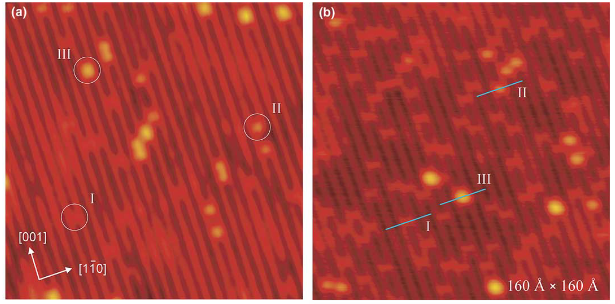
\includegraphics[width=.7\textwidth]{stm_end1.png}
\caption{Különböző módon kezelt TiO$_2$ felületek}
\end{figure}
\end{frame}

\begin{frame}
\begin{figure}
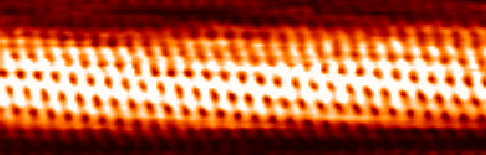
\includegraphics[width=.9\textwidth]{stm_end2.png}
\caption{Szén nanocsövek}
\end{figure}
\end{frame}

\section{Hivatkozások}
\begin{frame}
\frametitle{\secname}
\begin{thebibliography}{99}
\small
\bibitem{qd-eur}
\url{https://qd-europe.com/it/en/news/latest-updates/newsdetails/history-and-background-of-atomic-force-microscopy--1807/}
\bibitem{thor_afm}
\url{https://www.thorlabs.com/newgrouppage9.cfm?objectgroup_{}id=10756/}
\bibitem{cikk}
Andrea Alessandrini és Paolo Facci: \textit{AFM: a versatile tool in biophysics}
\bibitem{ibm_stm}
\url{https://www.ibm.com/ibm/history/ibm100/us/en/icons/microscope/}
\bibitem{nist_stm}
\url{https://www.nist.gov/pml/scanning-tunneling-microscope/scanning-tunneling-microscope-introduction}
\bibitem{cikk2}
S. Wendt et. al: \textit{Oxygen vacancies on TiO2(1 1 0) and their interaction with H2O and O2:\\A combined high-resolution STM and DFT study}
\end{thebibliography}
\end{frame}

\end{document}

% Linkek https://qd-europe.com/it/en/news/latest-updates/newsdetails/history-and-background-of-atomic-force-microscopy--1807/